\chapter{The Freeflow Runtime and Steve} \label{ch:flowpath}

To load a Steve application, a switch must expose a consistent application binary interface (ABI) that the Steve program can call to access switch resources and optimized operations.
To validate this approach, Steve targets a programmable, protocol independent, software data plane called Freeflow Virtual Machine (FFVM) \cite{freeflow_software}. 
FFVM virtualizes switch hardware as depicted in Figure \ref{fig:architecture}. 
FFVM provides a runtime environment which exposes switch resources to the Steve application through an ABI. 

Having a dedicated runtime environment provides Steve with two advantages.
First, the ABI exposed by the runtime environment provides consistent resource access across all devices, meaning code generation differences between devices is minimal.
Second, resource management is pushed into the data plane, making it completely opaque to the application. This way the application need not worry about discovering all resources on a device.
The Steve application also provides an interface so that the switch may use it to configure its pipeline, decode packets, and access event handlers.
The topic of this chapter will be describing these two interfaces.



%
%The Freeflow Virtual Machine (FFVM) is a software data plane that is programmable and protocol independent \cite{freeflow_software}. Freeflow provides a runtime environment (FFRT) for networking applications. FFRT is designed to abstract underlying hardware such as ports, memory, and flow tables. It exposes these resources through an interoperable ABI which can be used by almost any language. 
%
%Applications which target the FFVM ABI are called \emph{Freeflow managed applications}.
%These applications are dynamic link libraries (DLLs) designed to be loaded by FFVM.
%Their purpose is to program the data plane's packet processing pipeline by providing decoding logic and flow table configuration. They also act as the non-distributed controller for the Freeflow data plane. The architecture of this system is depicted in Figure \ref{fig:architecture}.

\begin{figure}[ht]
\centering
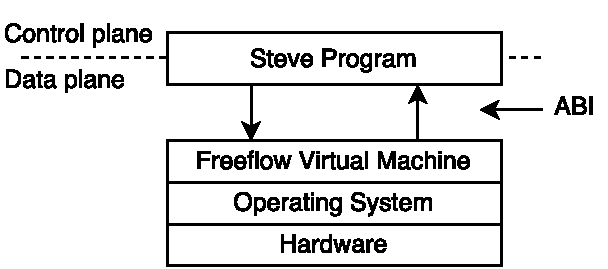
\includegraphics[scale=0.75]{architecture}
\caption{The FFVM architecture. FFVM virtualizes the underlying switch hardware and switch OS. Steve programs are loaded by FFVM and instantiates the data plane's pipeline. The Steve program also serves as the device's controller.}
\label{fig:architecture}
\end{figure}


%These other programs, known as \textit{pipeline applications}, contain all the packet processing logic. Packet decoders, flow table configuration details, flow entry definitions, and exceptional event handlers are contained inside these pipeline applications.
%Freeflow is designed to load these pipeline applications which are dynamic link libraries confirming to a certain Freeflow specification. Encapsulating all this functionality into these applications makes the data plane incredibly modular. The entire behavior of the data plane can instantly change by removing one application and loading another without having to stop and recompile the data plane's software. For example, in seconds, a Freeflow data plane instance can go from being an L2 switch to and L3 switch just by changing applications. 

%For now, the Steve compiler is specifically tailored toward compiling Freeflow pipeline applications. This chapter will focus on Freeflow, its interactions with Steve, and how Steve applications use the Freeflow API in its packet processing pipeline. 

\section{Freeflow ABI} \label{fp:dp_interface}

The Freeflow runtime environment exposes a set of \emph{system calls} through compiled functions which allow applications to gain controlled access to switch resources. Table \ref{tbl:Freeflow_api} summarizes the common usage of the library.
Specifically, the ABI provides access to flow table allocation, flow entry manipulation, and ports.

\begin{table}[ht]
\caption{The Freeflow ABI that may be used by applications. The ABI and its function implementations are subject to change, so specific parameters and return types are not given.}
\begin{center}
\begin{tabular}{| p{0.4\linewidth} | p{0.55\linewidth} |}
\hline
Interface Functions & Description \\

% % % % % % % % % % % % % % %
\hline
\texttt{ff\_output(context, portid)} 

\texttt{ff\_drop(context)}
& 
Creates a copy of the packet stored with the context and forwards it to the port with the given id. \\
\hline 
% % % % % % % % % % % % % % % 

\texttt{ff\_goto\_table(context, table, key)} & 
Sends a context to be matched against a given table. The application is responsible for telling the data plane which fields must be extracted from the context and turned into a query key. \\

\hline
% % % % % % % % % % % % % % %

\texttt{ff\_create\_table(dataplane, key\_width, size, type)} &
Instructs a data plane instance to construct a flow table and return a handle to that flow table. The application is responsible for informing the data plane of the key width, the maximum number of flow entries (size), and the match pattern (type). \\
\hline

% % % % % % % % % % % % % % %

\texttt{ff\_insert\_flow(table, actions, key, info)}

\texttt{ff\_insert\_miss(table, actions, info)}

&

Allows for adding initial flow entries, new flow entries, and miss case flow entries to a given table. \\
\hline
% % % % % % % % % % % % % % % 

\texttt{ff\_remove\_flow(table, key)}

\texttt{ff\_remove\_miss(table)} &

Allows for deleting flow entries with certain match fields, or for removing the miss case. \\

\hline

% % % % % % % % % % % % % % % 

\texttt{ff\_raise\_event(context, handler)} &
Requests that the runtime queues up a context and an event handler on the controller port. The controller then executes the event handlers as it receives the contexts. Execution may not be immediate. \\
\hline

% % % % % % % % % % % % % % %

\texttt{ff\_port\_id\_is\_up(portid)}

\texttt{ff\_port\_id\_is\_down(portid)} &

Returns true or false depending on whether a port is up or down. \\

\hline

\end{tabular}
\end{center}
\label{tbl:Freeflow_api}
\end{table}

\section{Steve Applications} \label{fp:app_interface}

The Steve application is a dynamic link library (or shared object library). The Steve application provides an interface which a switch can use to modify its network function.
Specifically, the switch uses this interface to configure its flow tables, access decoders, initiate pipeline processing on a context, or execute event handlers.
Table \ref{tbl:steve_api} summarizes the application interface.

\begin{table}[ht]
\caption{The application interface. All Freeflow loadable applications must provide this interface.}
\begin{center}
\begin{tabular}{| p{0.3\linewidth} | p{0.65\linewidth} |}
\hline
Interface Functions & Functionality \\

\hline

\texttt{ff\_load(dataplane)} & This function is used for configuration when an application gets loaded. Freeflow passes a data plane handle to this function. This function then calls the Freeflow ABI to set up flow tables and flow entries. \\

\hline

\texttt{ff\_unload(dataplane)} & This function releases all dataplane resources allocated by the application. \\

\hline

\texttt{ff\_process(context)} & Freeflow sends contexts through this function to start pipeline processing. The application's logic will dictate which decoders and tables are used. Once the application finishes execution, Freeflow executes egress processing described in Section \ref{egress_desc}. \\

\hline
Event Handlers & Event handlers may vary in name, but all accept a context as a parameter. Whenever an event is raised, an event handler with the same name is executed.\\
\hline

\texttt{ff\_start(dataplane)}
\texttt{ff\_stop(dataplane)}
 & These are used to start and stop the delivery of events. \\
 
\hline

\end{tabular}
\end{center}
\label{tbl:steve_api}
\end{table}

%\section{Context Data Structure as a Message Format}
%
%The context data structure described in Section \ref{context_desc} can be thought of as a binary message between the data plane and the Steve application. 
%The context data structure is allocated by the data plane and is passed off to the application which uses it to convey decoding state and metadata.
%The application sends this context back to the data plane during table matching and egress processing. The data plane then reads back the information it needs from the context.
%As a consequence, both the Freeflow runtime environment and the Steve application must know about the same data structure. 
%
%\section{Application Loading and Runtime Configuration} \label{config_guide}
%
%To load a pipeline application, one must write a Freeflow driver which finds and dynamically links against the pipeline application binary. This driver is implemented in C++ (the same language Freeflow is implemented in).
%The driver is responsible for the following operations using the Freeflow runtime library:
%
%\begin{enumerate}
%\item \textit{Port discovery.} The driver will discover all necessary ports on the system and manage receiving and forwarding through them.
%
%\item \textit{Application loading.} The driver will fetch and link in the Steve application.
%
%\item \textit{Configuration}. The driver will call the Steve application's \texttt{configure} function described in Table \ref{tbl:steve_api}. Steve will make requests for tables and initial flow entries using the Freeflow API. The Steve application will ask for a table with a certain ID number, maximum flow entry size, and key width. Freeflow will allocate such a table and return a handle to the table back to the Steve application. Once the handle is received, the Steve application will provide initial flow entries to be inserted into the table.
%
%\item \textit{Ingress processing}. Drivers must perform the ingress processing phase described in Section \ref{ingress_desc}. The driver will handle receiving packets on ports and allocating the context data structures for them.
%
%\item \textit{Pipeline processing.} Freeflow will begin sending contexts to the Steve application for pipeline processing through the \texttt{process} function described in Table \ref{tbl:steve_api}.
%
%\item \textit{Egress processing.} Once the \texttt{process} function completes, the driver will handle the egress processing phase described in Section \ref{egress_desc}.
%\end{enumerate}

\section{Steve Compilation} \label{compile}

Steve compilation is a three stage process.
In the first stage, high-level network-specific syntax is lowered into primitive code elements such as functions, function calls, variables, system intrinsics, etc.
In the second stage, Steve is compiled into LLVM IR \cite{llvm_webpage}. The LLVM IR is linked against the Steve runtime library which contains the context data structure. The context data structure is kept in an independent library so that different context formats may be easily swapped out depending on the target architecture.
In the last stage, the LLVM IR is compiled by the LLVM optimizing compiler into assembly code which is assembled into the DLL.

\section{Application Lifetime} \label{lifetime}

When FFVM loads a Steve application library, it calls \texttt{ff\_load} which initializes flow tables. Once loading is complete, FFVM calls the \texttt{ff\_process} function to dispatch a context to the first decoder. 
FFVM will use \texttt{ff\_start} and \texttt{ff\_stop} to start and stop the delivery of events to the application.
When FFVM wants to remove the application, it calls \texttt{ff\_unload} which releases all resources requested by the application.